La spirale d'Ulam consiste à avoir une grille de nombre remplie en forme de spirale et de marquer les nombres premiers.
\begin{figure}[!h]
\begin{center}
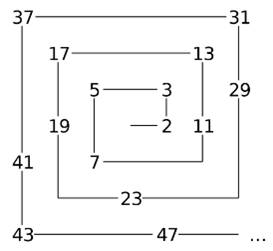
\includegraphics[scale=0.8]{images/spirale_explication.jpg}
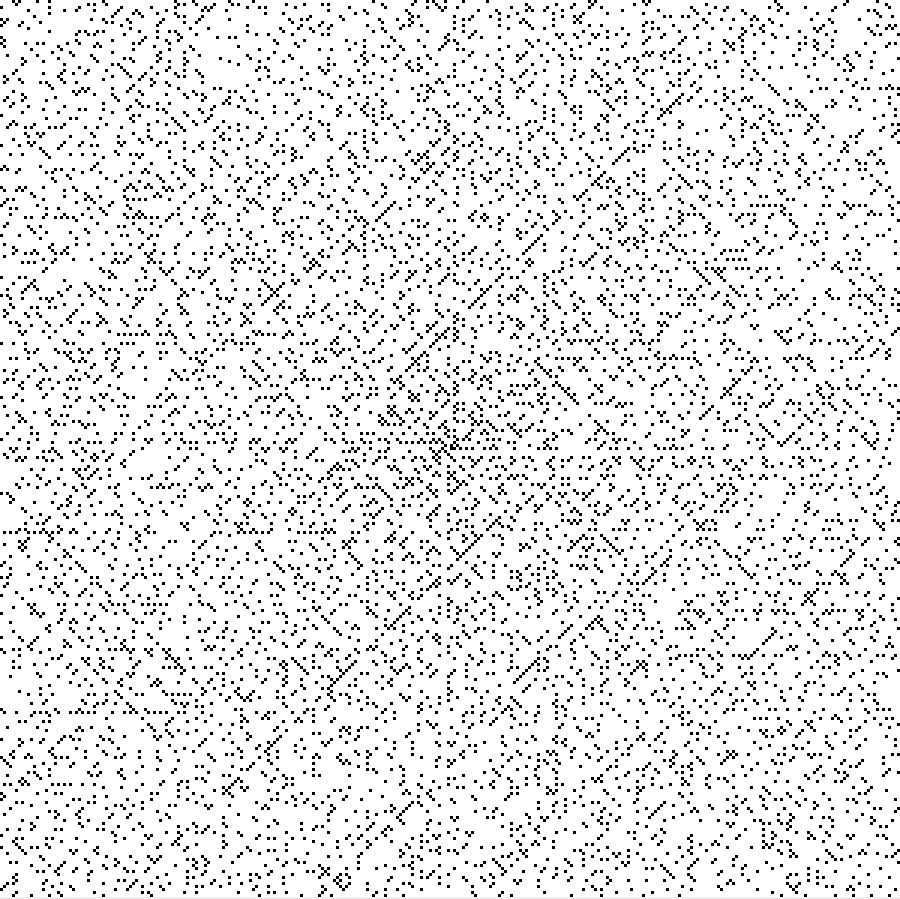
\includegraphics[scale=0.3]{images/spirale_explication.PNG}
\end{center}
\caption{Spirale d'Ulam}
\end{figure}

\subsubsection{Réalisation}
Nous avons réalisé cette spirale en Java en utilisant la bibliothèque Swing. Pour la partie modèle, nous avons séparé le problème en deux classes : une qui modélise la grille (\textbf{Board}) et l'autre représentant un curseur (\textbf{Cursor}) en abstrait, qui pointera sur la case que la grille doit remplir et qui s'occupera de l'ordre de remplissage. Une implémentation de cette classe abstraite est \textbf{SpiralCursor} qui se déplacera en forme de spirale dans la grille (on pourrait bien évidemment envisager différents types de remplissage et il suffirait d'ajouter une nouvelle implémentation de curseur).\\ 
Un curseur s'utilise un peu de la même manière qu'un \textbf{Iterator} en Java, il prend en argument une grille et il se place à une certaine coordonnée et direction de départ. Il possède deux principales méthodes, \textbf{canMove} qui va tester si la case de la grille est déjà remplie à une distance d'une case dans la direction où le curseur est tourné, la seconde méthode est \textbf{next} qui fait avancer le curseur d'une case dans la direction vers laquelle il est tourné.\\

\begin{figure}[H]
\begin{center}
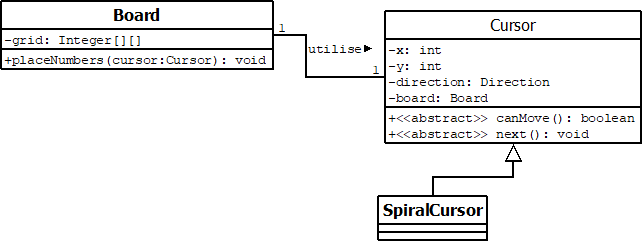
\includegraphics[scale=0.5]{images/dia_spirale.png}
\end{center}
\caption{Diagramme de classe pour la spirale d'Ulam}
\end{figure}

Ensuite, pour la partie graphique, nous avons simplement fait une fenêtre qui possède un \textbf{JPanel} sur lequel on va dessiner notre grille en ne remplissant que les cases qui possèdent un nombre premier en noir.

\begin{figure}[H]
\begin{center}
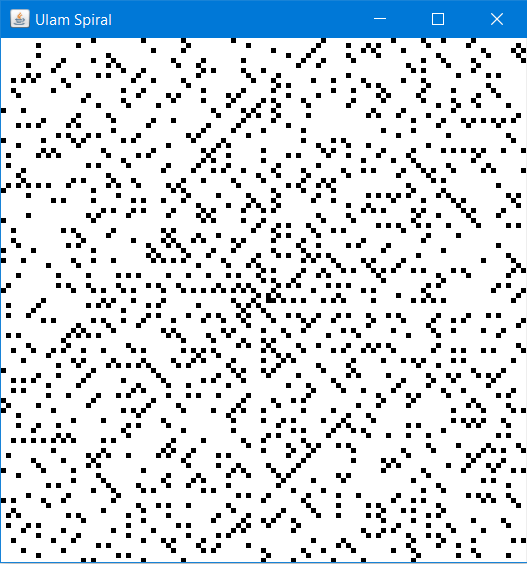
\includegraphics[scale=0.5]{images/swing_spirale.PNG}
\end{center}
\caption{Interface graphique de la spirale d'Ulam en Swing}
\end{figure}

Le test de primalité utilisé dans cette partie est simplement un parcours de 3 à $\sqrt{n} + 1$ avec un pas de deux. Il n'était pas nécessaire d'implémenter l'exponentiation modulaire car nous avons qu'une petite partie de nombre premiers donc la différence de temps aurait été faible.\\
\newpage
\lstinputlisting[language=Java, firstline=14, lastline=31]{../java/src/utilitaire/MyMath.java}

\subsubsection{Observations}
En prenant certaines valeurs de départ pour le remplissage de la spirale, on peut remarquer un alignement de nombres premiers, par exemple pour 41 on retrouve une ligne diagonale et pour 104 on peut apercevoir deux alignements parallèles en diagonale ainsi qu'une sorte de grand quadrillage.

\begin{figure}[H]
\begin{center}
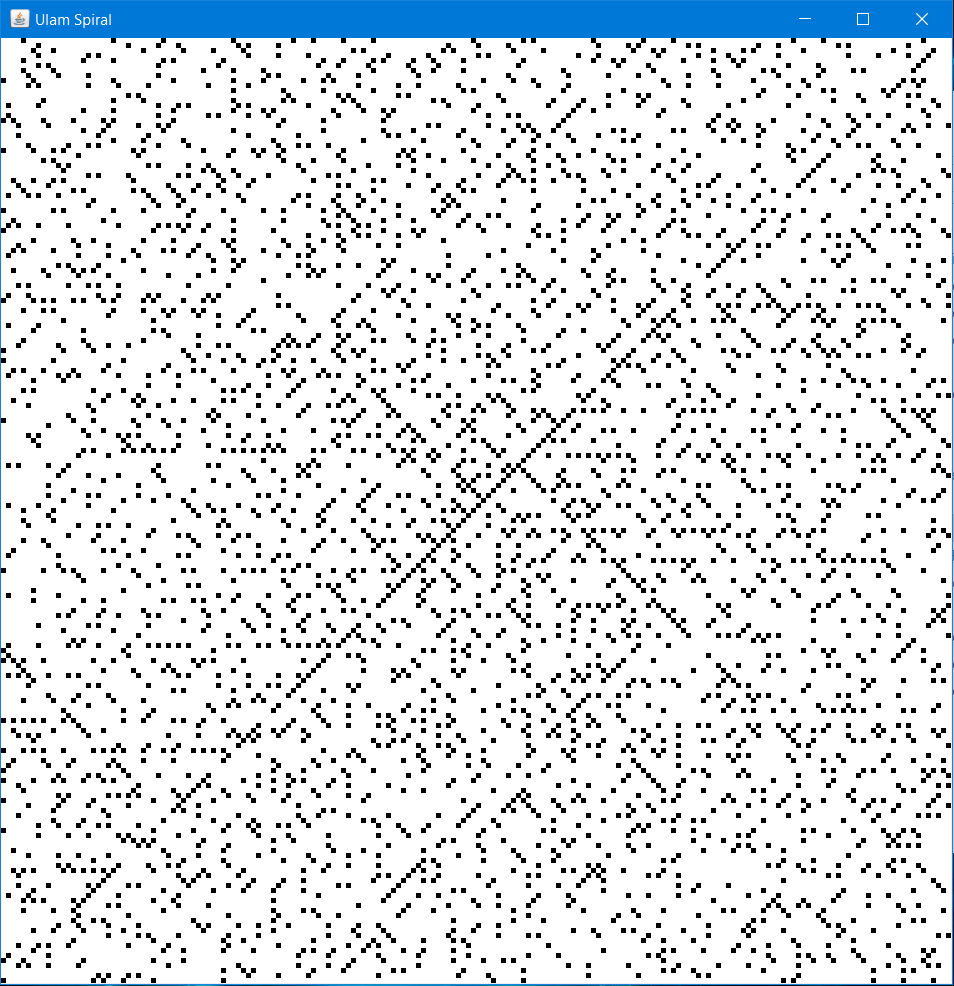
\includegraphics[scale=0.3]{images/spirale_41.PNG}
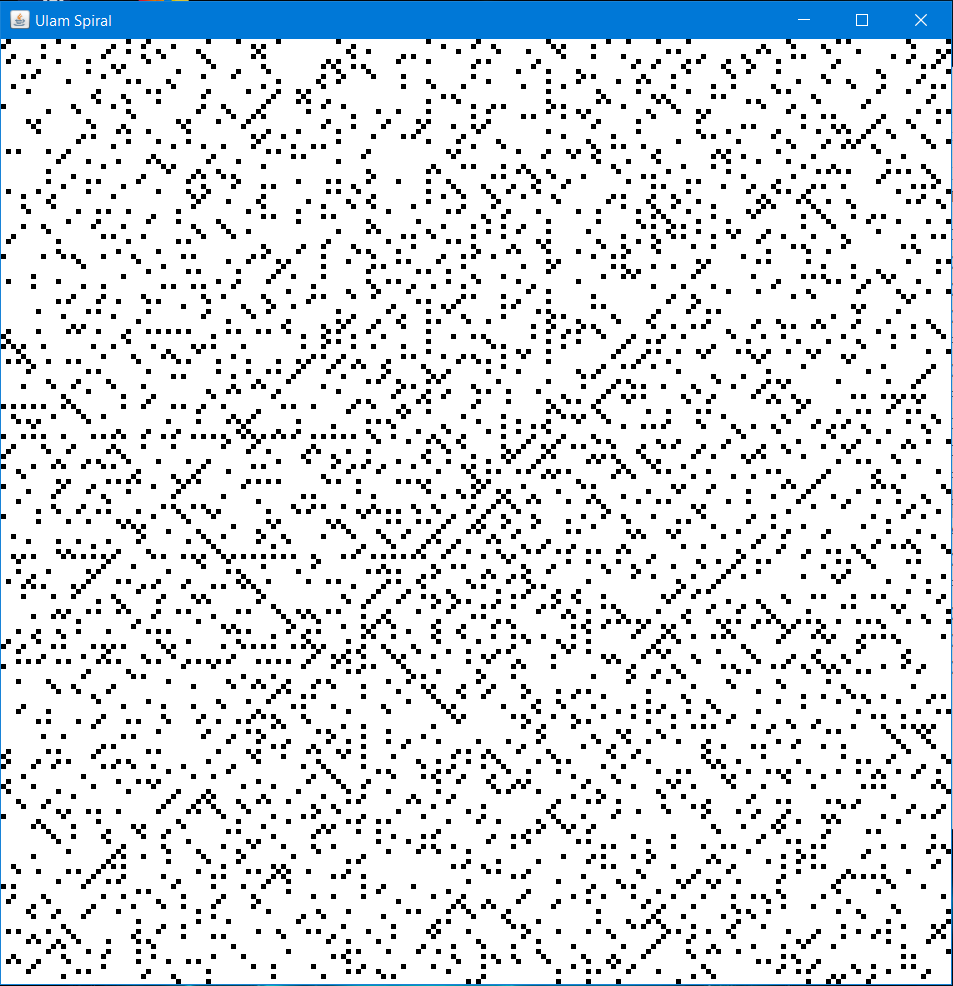
\includegraphics[scale=0.3]{images/spirale_104.PNG}
\end{center}
\caption{Spirale d'Ulam avec 41 (à gauche) et 104 (à droite) pris comme nombre de départ}
\end{figure}

Sachant qu'il y a une infinité de nombres premiers et que leur fréquence diminue logarithmiquement à mesure qu'on tend vers l'infini, c'est tout naturellement qu'on constate que les cases de nombres premiers sont plus condensées en commençant la spirale avec 1 qu'avec un plus grand nombre comme 1548468615.

\begin{figure}[H]
\begin{center}
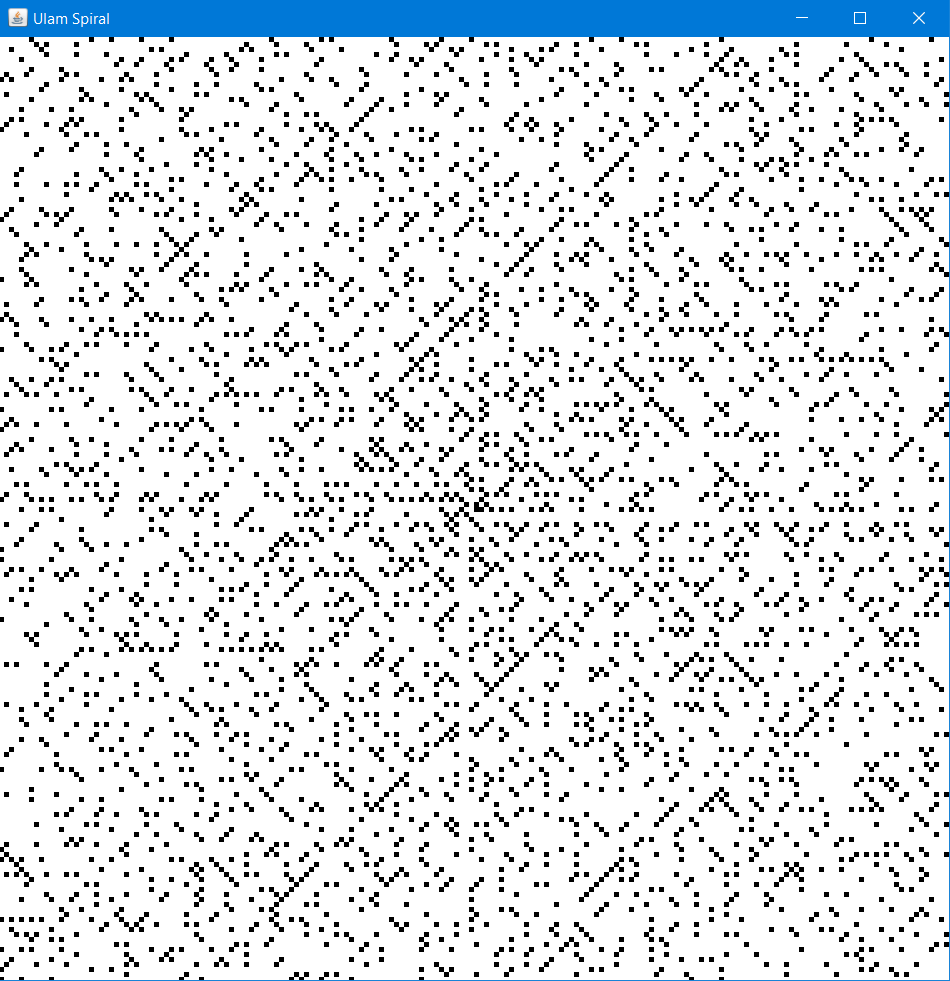
\includegraphics[scale=0.3]{images/spirale_1.PNG}
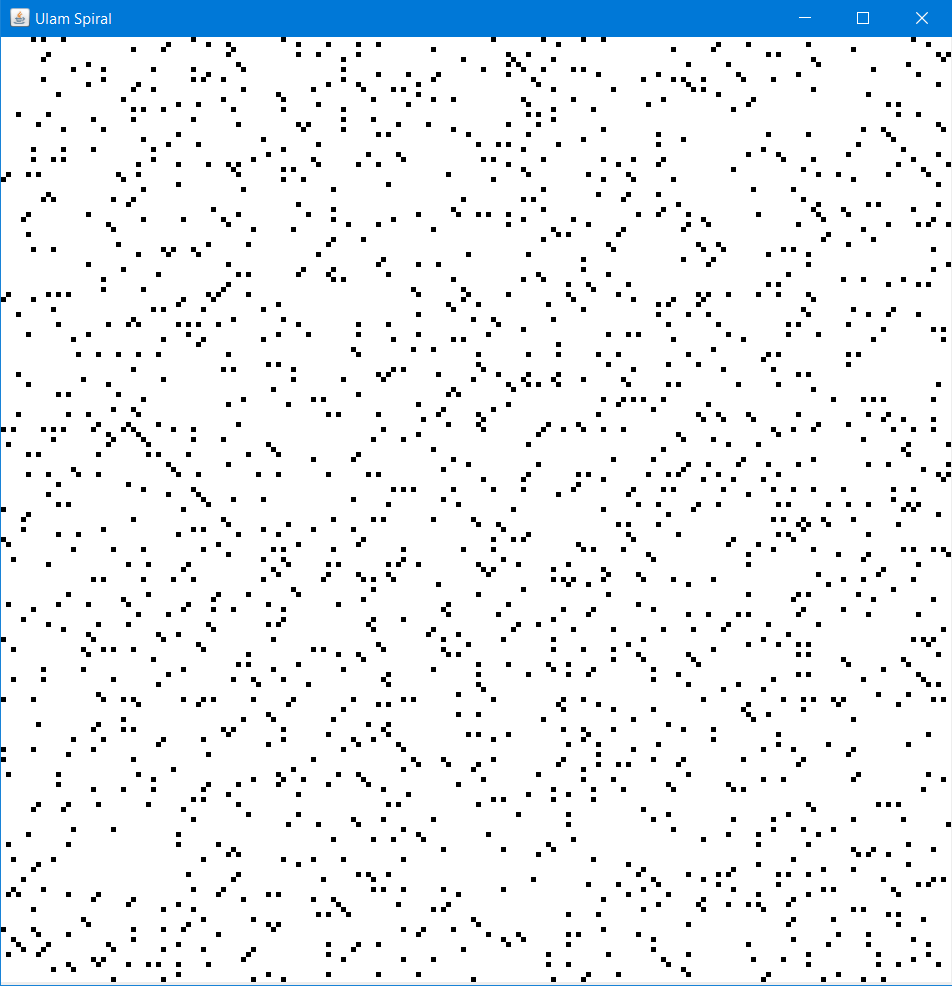
\includegraphics[scale=0.3]{images/spirale_grandNB.PNG}
\end{center}
\caption{Spirale d'Ulam avec 1 et 1548468615 pris comme nombre de départ}
\end{figure}


